% !TEX root = ../main.tex

\section{Blend3 feedstock results}

Biomass composition, batch reactor conversion, and EFR pyrolysis yields for the Blend3 feedstock are discussed in this section.

\subsection{Biomass composition}

Several approaches were investigated to characterize the Blend3 feedstock for use with the Debiagi pyrolysis kinetics. These approaches are explored below as Cases 1 through 5. Ultimate analysis data is used for Cases 1 and 2 while chemical analysis data is used for Cases 3, 4, and 5.

\textbf{Case 1:} Using the ultimate analysis data from Table \ref{tab:blend3-ult}, the dry and dry ash-free (daf) bases were calculated as shown in Table \ref{tab:blend3-ult-bases}. The dry ash-free basis in terms of the C, H, and O fractions are used for the biomass characterization procedure discussed in the Debiagi et al. 2015 \cite{Debiagi-2015}. To use this approach for the Blend3 feedstock, a C mass fraction of 53.16\% and H mass fraction of 5.67\% was used (see last column in Table \ref{tab:blend3-ult-bases}). Also from the characterization procedure, the default splitting parameters of $\alpha = 0.6$, $\beta = 0.8$, $\gamma = 0.8$, $\delta = 1.0$, and $\epsilon = 1.0$ which do not account for extractives were used for Case 1.

Results from this characterization are shown in Figure \ref{fig:blend3-biocharact-ult} and the associated biomass composition is given in Table \ref{tab:blend3-biocomp}. While this approach is useful for limited feedstock data, its accuracy is questionable when compared to experimental measurements. For example, chemical analysis of the Blend3 feedstock provides a lignin composition of approximately 29\% whereas the characterization method using ultimate analysis data estimates a total lignin composition greater than 59\%.

\begin{table}[H]
    \centering
    \caption{Ultimate analysis bases for the Blend3 feedstock. Mass percent values are given for as-received (ar), dry, and dry ash-free (daf) basis.}
    \label{tab:blend3-ult-bases}
    \begin{tabular}{lrrrr}
        \toprule
        Element & \% ar & \% dry & \% daf & \% daf \\
        \midrule
        C        & 49.52 & 52.70 & 53.06 & 53.16 \\
        H        & 5.28  & 5.62  & 5.66  & 5.67  \\
        O        & 38.35 & 40.82 & 41.10 & 41.17 \\
        N        & 0.15  & 0.16  & 0.16  &       \\
        S        & 0.02  & 0.02  & 0.02  &       \\
        ash      & 0.64  & 0.68  &       &       \\
        moisture & 6.04  &       &       &       \\
        \bottomrule
    \end{tabular}
\end{table}

\begin{figure}[H]
    \centering
    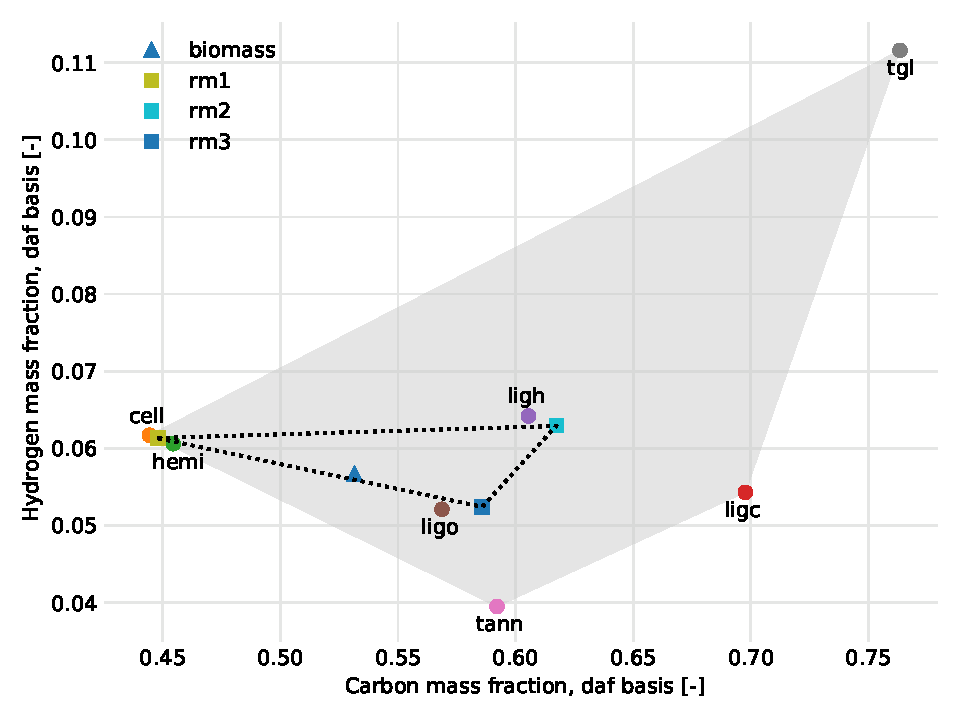
\includegraphics[width=0.8\textwidth]{figures/blend3-biocharact-ult.pdf}
    \caption{Characterization of the Blend3 feedstock using ultimate analysis data. Reference mixtures (rm) are labeled with square markers.}
    \label{fig:blend3-biocharact-ult}
\end{figure}

\textbf{Case 2:} To improve the Blend3 characterization based on ultimate analysis data, the splitting parameters were adjusted to account for extractives in the feedstock by using $\alpha = 0.56$, $\beta = 0.6$, $\gamma = 0.6$, $\delta = 0.78$, and $\epsilon = 0.88$. Also, since the uncertainty in the ultimate analysis data is unknown (see Table \ref{tab:blend3-ult}) the carbon mass fraction was adjusted to 51\% and the hydrogen mass fraction to 6\%.

Results from the Case 2 characterization adjustments are presented in Figure \ref{fig:blend3-biocharact-ultmod} while the biomass composition is given in Table \ref{tab:blend3-biocomp}. The estimated cellulose, hemicellulose, and total lignin are near the measured values for these components. By adjusting the splitting parameters, reasonable biomass compositions can be determined from the ultimate analysis data; however, it remains to be seen if the tannin and triglyceride fractions are reasonable.

\begin{figure}[H]
    \centering
    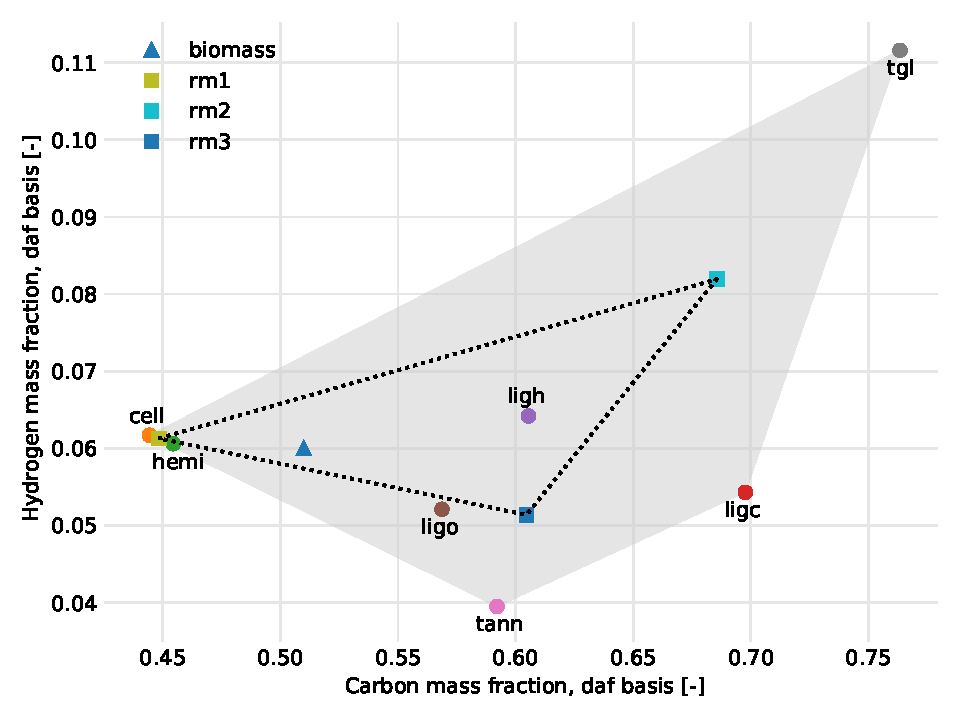
\includegraphics[width=0.8\textwidth]{figures/blend3-biocharact-ultmod.pdf}
    \caption{Characterization of the Blend3 feedstock using modified ultimate analysis data and adjusting the splitting parameters to account for extractives. Reference mixtures (rm) are labeled with square markers.}
    \label{fig:blend3-biocharact-ultmod}
\end{figure}

\textbf{Case 3:} The next approach to characterize the Blend3 feedstock, was to use chemical analysis data (see Table \ref{tab:blend3-chem-analysis}) to determine the biomass composition. For this case, the cellulose is represented by glucan while hemicellulose is comprised of xylan, mannan, galactan, arabinan, free fructose, free glucose, and sucrose. The measurement technique to determine the lignin components is unknown; therefore, one third of the lignin represents each of the carbon, hydrogen, and oxygen-rich fractions. Tannins are represented by acetyl, water extractives, and ethanol extractives while ash is the non-structural and structural inorganics. Triglycerides were not considered for this case. The Case 3 biomass composition based on the chemical analysis measurements is given in Table \ref{tab:blend3-biocomp}.

\textbf{Cases 4 and 5:} Two more Blend3 feedstock compositions were modeled to investigate the compositional effect on pyrolysis yields. The Case 4 composition regards the extractives as all triglycerides, not tannins. This is motivated by the sensitivity analysis where triglycerides had the largest impact on liquid yields. Case 5 divides all the lignin equally into the H and O fractions thus ignoring the C fraction. This was also motivated by the sensitivity analysis where the carbon-rich lignin had the greatest effect on solids production compared to the other lignin fractions. See Table \ref{tab:blend3-biocomp} for the biomass compositions that correspond to Cases 4 and 5.

\begin{table}[H]
    \centering
    \caption{Biomass composition for the Blend3 feedstock. Values are reported as mass percent on a dry ash-free basis (\% daf). Cases 1 and 2 rely on ultimate analysis data while Cases 3, 4, and 5 use chemical analysis data.}
    \label{tab:blend3-biocomp}
    \begin{tabular}{lrrrrrr}
        \toprule
        Biomass composition & Exp. & Case 1 & Case 2 & Case 3 & Case 4 & Case 5 \\
        \midrule
        cellulose     & 39.91 & 26.38 & 39.24 & 39.19 & 39.19 & 39.19 \\
        hemicellulose & 23.26 & 14.33 & 25.12 & 23.26 & 23.26 & 23.26 \\
        lignin        & 29.66 & --    & --    & --    & --    & --    \\
        lignin-c      & --    & 7.84  & 8.57  & 9.89  & 9.89  & 0     \\
        lignin-h      & --    & 5.27  & 3.11  & 9.89  & 9.89  & 14.83 \\
        lignin-o      & --    & 46.18 & 18.00 & 9.89  & 9.89  & 14.83 \\
        tannins       & 7.88  & 0     & 2.95  & 7.88  & 0     & 0     \\
        triglycerides & 0     & 0     & 3.01  & 0     & 7.88  & 7.88  \\
        \bottomrule
    \end{tabular}
\end{table}

\subsection{Batch reactor conversion}

To understand the time scales associated with the pyrolysis kinetics, the batch reactor model was implemented with the Case 1, 2, and 3 biomass compositions from Table \ref{tab:blend3-biocomp}. The final concentrations in the batch reactor after 10 seconds of reaction at 500$^{\circ}$C are shown in Table \ref{tab:blend3-batch-final}. These results do not utilize the thermo data for the Debiagi kinetics; therefore, they neglect exothermic or endothermic effects from heats of reactions. As the table shows, concentrations vary considerably based on the initial biomass composition. Therefore, it is essential to correctly characterize the biomass composition to obtain reasonable results from the Debiagi pyrolysis kinetics.

\begin{table}[H]
    \centering
    \caption{Final batch reactor concentrations for the Blend3 feedstock without thermodynamic effects. Values reported as \% mass.}
    \label{tab:blend3-batch-final}
    \begin{tabular}{lrrr}
        \toprule
        Final concentration & Case 1 & Case 2 & Case 3 \\
        \midrule
        gases         & 18.40 & 15.93 & 14.99 \\
        liquids       & 40.08 & 55.79 & 52.51 \\
        solids        & 20.84 & 16.25 & 20.92 \\
        metaplastics  & 20.68 & 12.04 & 11.59 \\
        \bottomrule
    \end{tabular}
\end{table}

For the Blend3 biomass composition based on the chemical analysis data (Case 3), evolutions of the gas, liquid, solid, and metaplastic species are shown in Figures \ref{fig:blend3-case3-gases-liquids} and \ref{fig:blend3-case3-solids-meta}. The results are generated with and without using thermodynamic data for the Debiagi kinetics. Gaseous species remain under 8\% for both thermodynamic scenarios. Liquid species reach steady-state concentrations within 2.5 seconds without thermo but continue to increase when thermodynamics are applied. Solid species except for tannins fully devolatilize within 10 seconds without thermodynamics but never fully convert when thermo data is utilized. Metaplastic species reach steady-state concentrations without thermodynamics but continue to devolatilize when thermodynamics are accounted for. The differences between the conversions seen with and without thermodynamic effects is due to the difference in temperature applied to the reaction rates during the two scenarios.

\begin{figure}[H]
    \makebox[\textwidth][c]{
        \begin{subfigure}{1.4\textwidth}
            \centering
            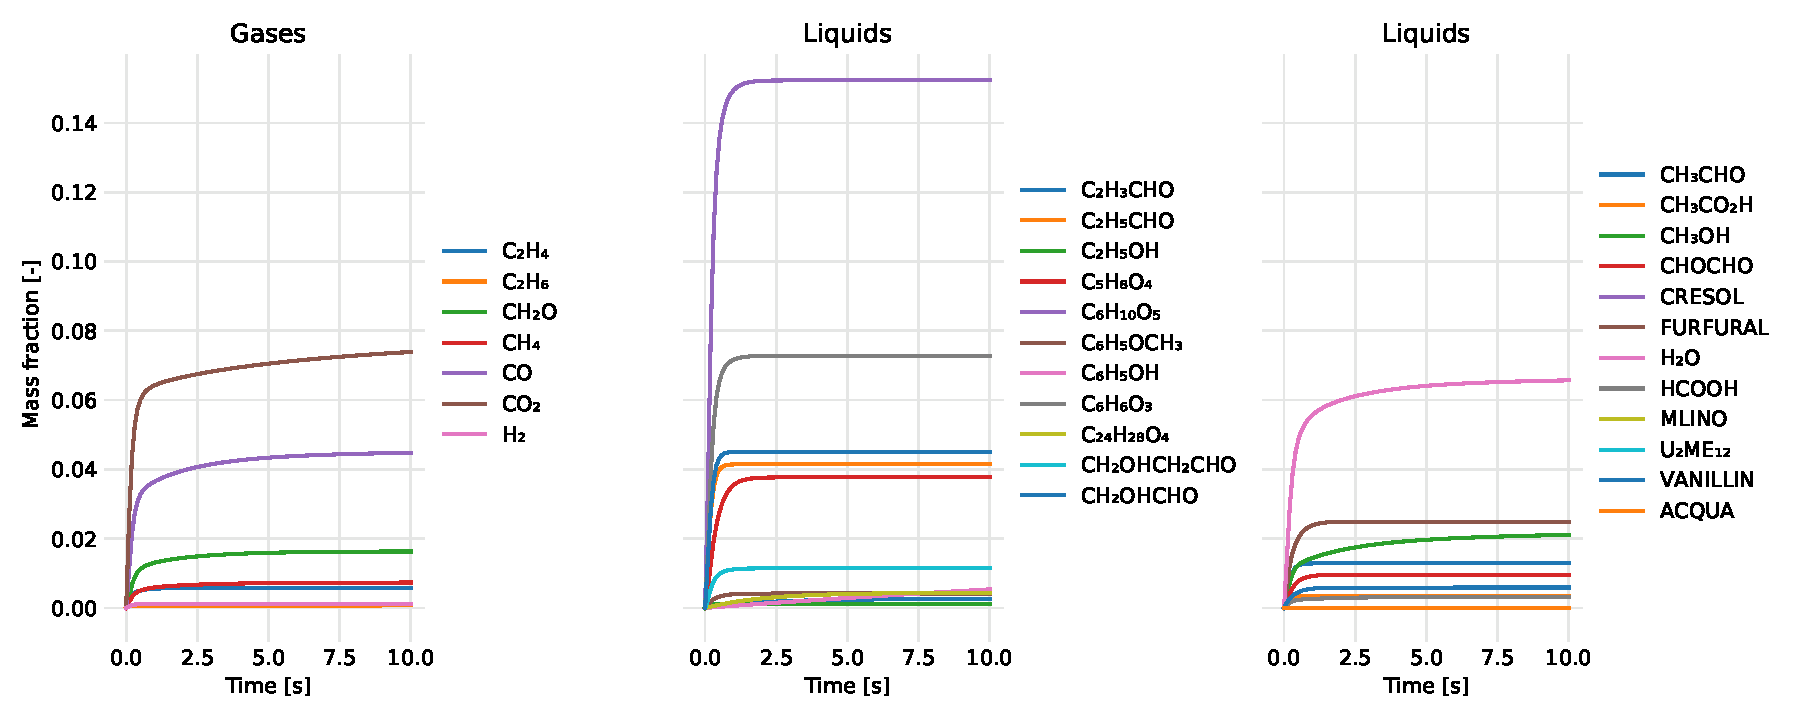
\includegraphics[width=\textwidth]{figures/blend3-case3-gases-liquids.pdf}
            \caption{Without thermodynamics.}
        \end{subfigure}
    }
    \makebox[\textwidth][c]{
        \begin{subfigure}{1.4\textwidth}
            \centering
            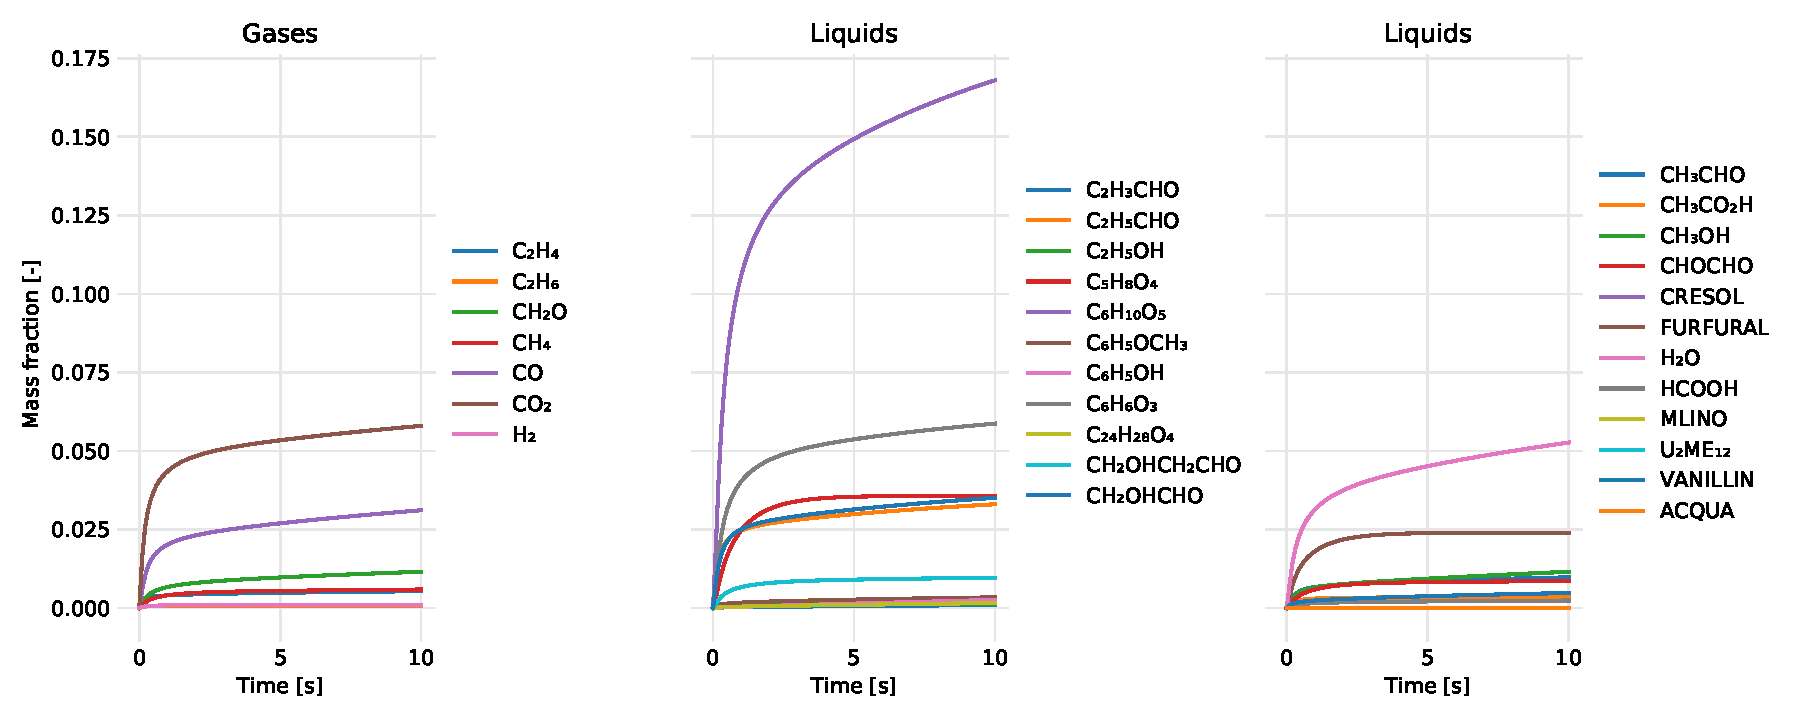
\includegraphics[width=\textwidth]{figures/blend3-case3-gases-liquids-thermo.pdf}
            \caption{With thermodynamics.}
        \end{subfigure}
    }
    \caption{Batch reactor gas and liquid concentrations for Blend3 feedstock based on Case 3 biomass composition.}
    \label{fig:blend3-case3-gases-liquids}
\end{figure}

\begin{figure}[H]
    \begin{subfigure}{\textwidth}
        \centering
        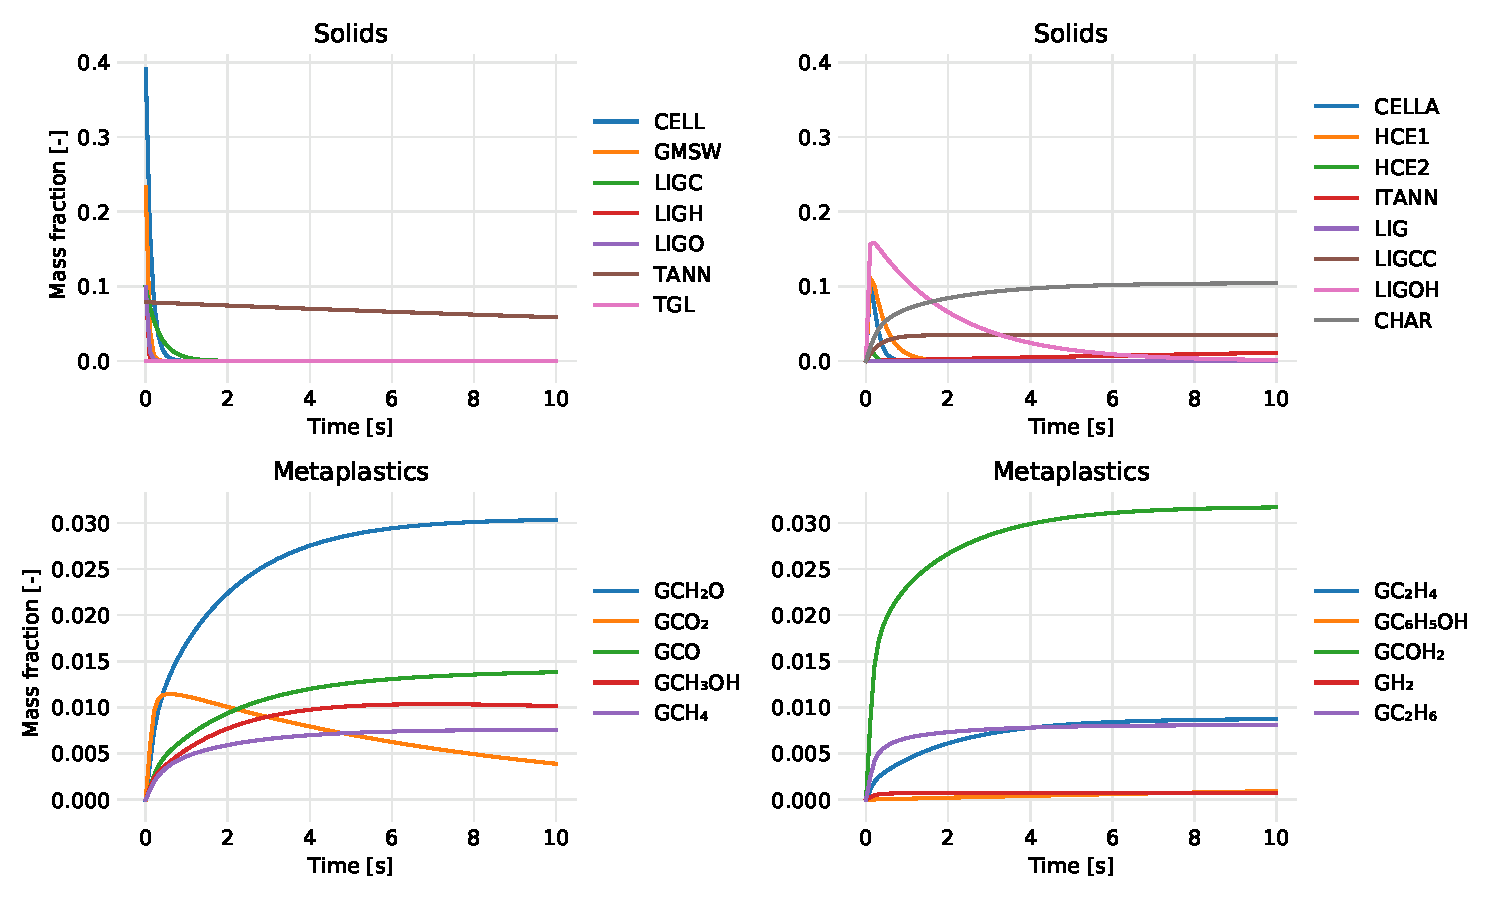
\includegraphics[width=\textwidth]{figures/blend3-case3-solids-meta.pdf}
        \caption{Without thermodynamics.}
    \end{subfigure}
    \begin{subfigure}{\textwidth}
        \centering
        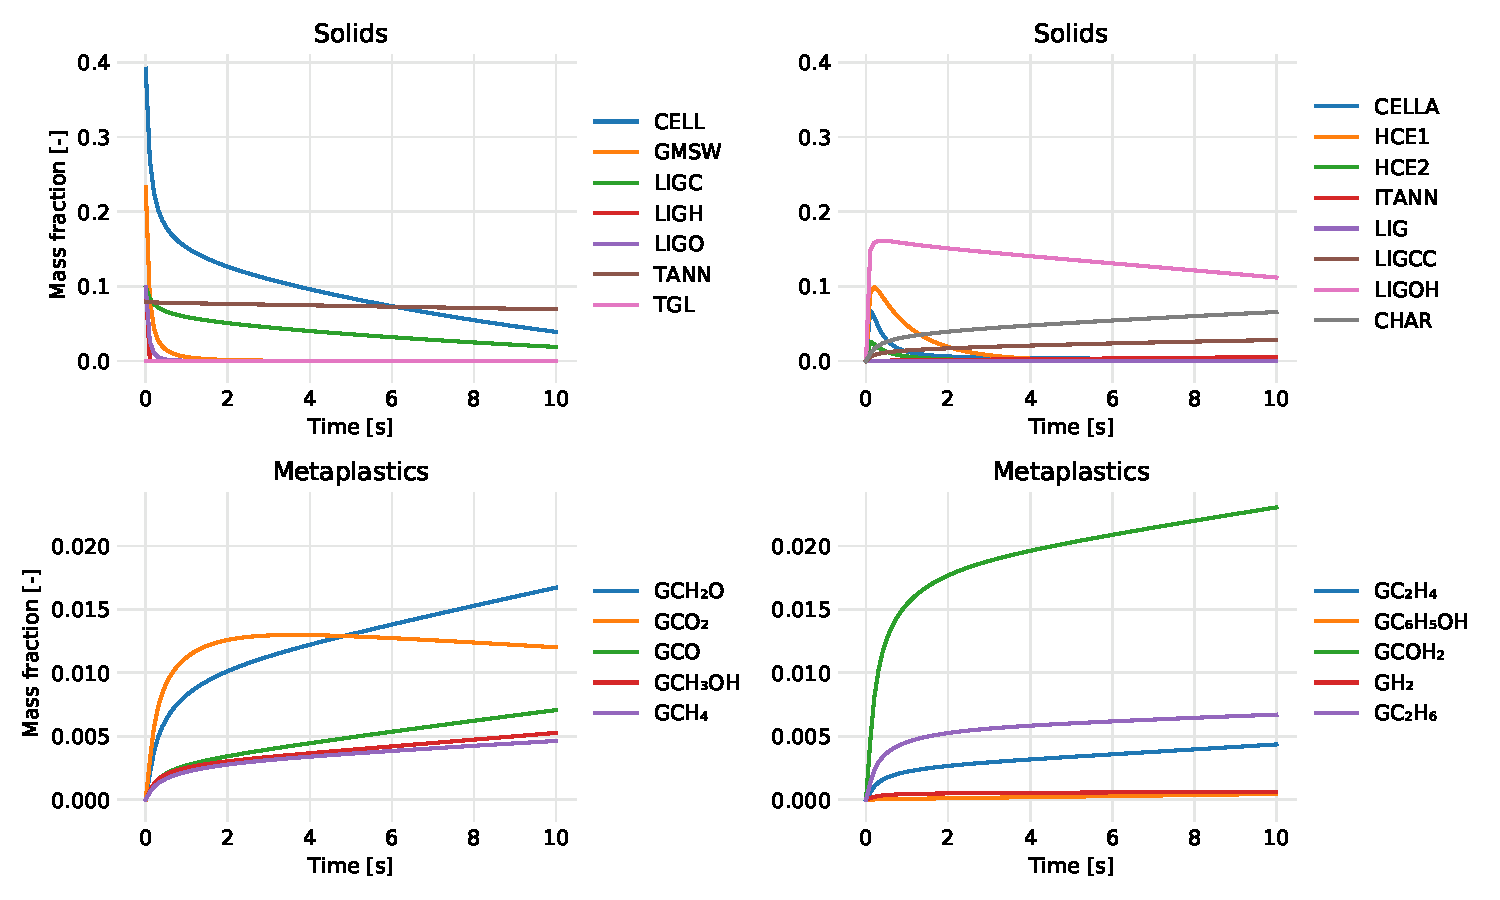
\includegraphics[width=\textwidth]{figures/blend3-case3-solids-meta-thermo.pdf}
        \caption{With thermodynamics.}
    \end{subfigure}
    \caption{Batch reactor solid and metaplastic concentrations for Blend3 feedstock based on Case 3 biomass composition.}
    \label{fig:blend3-case3-solids-meta}
\end{figure}

A comparison of the batch reactor results for total gas, liquid, solid, and metaplastic species is given in Figure \ref{fig:blend3-case3-phases-temp} along with the batch reactor temperature profile. Without thermodynamic effects, temperature in the reactor is constant at 500$^{\circ}$C and pyrolysis is mostly complete within 2 seconds. The main pyrolysis product in the reactor is the liquid species. Including thermodynamic effects, pyrolysis is still occuring at 10 seconds and a large amount of solid species remain in the batch reactor. Also, the reactor temperature decreases to 680 K (407$^{\circ}$C) suggesting an overall endothermic pyrolysis process. The metaplastic species are prominent during the entire process; therefore, their contribution to the total solids concentration is considerable at the given operating conditions.

\begin{figure}[H]
    \begin{subfigure}{\textwidth}
        \centering
        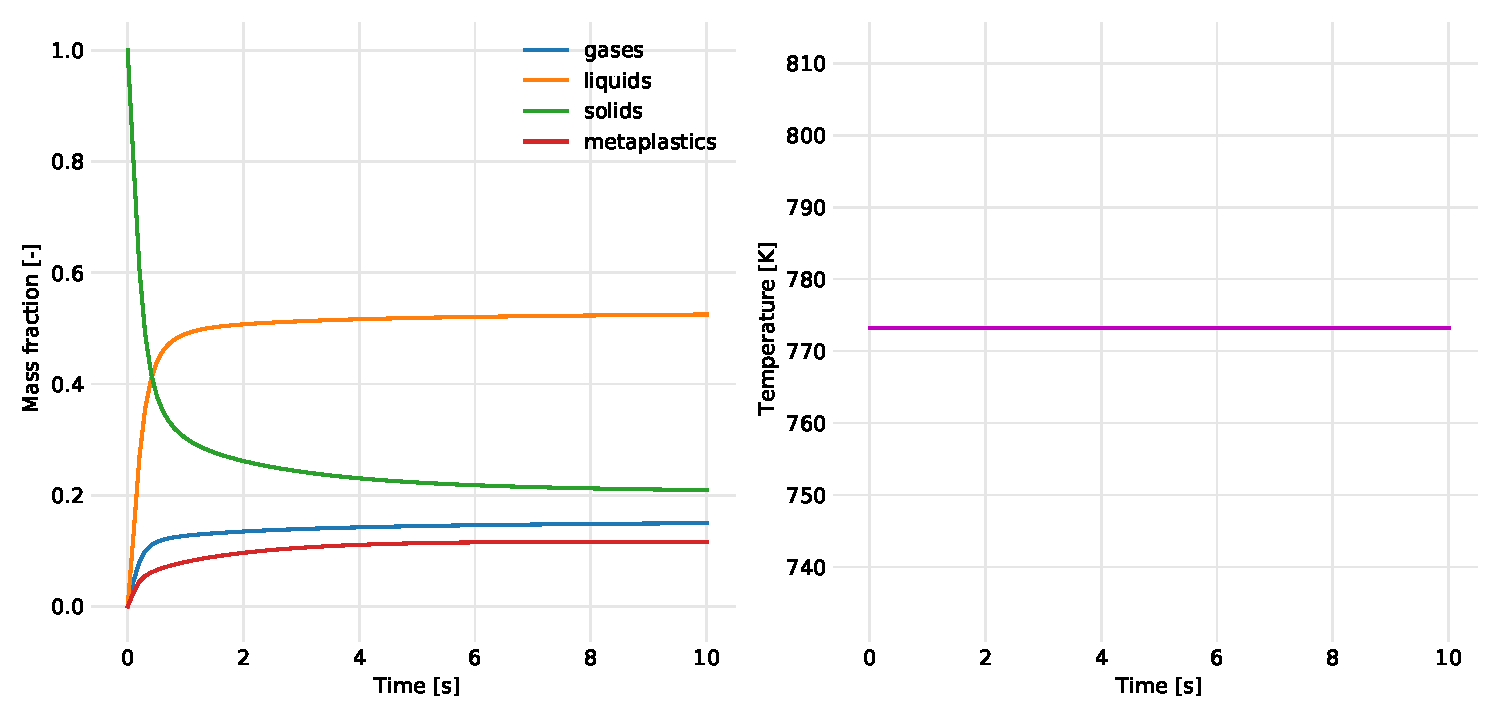
\includegraphics[width=\textwidth]{figures/blend3-case3-phases-temp.pdf}
        \caption{Without thermodynamics.}
    \end{subfigure}
    \begin{subfigure}{\textwidth}
        \centering
        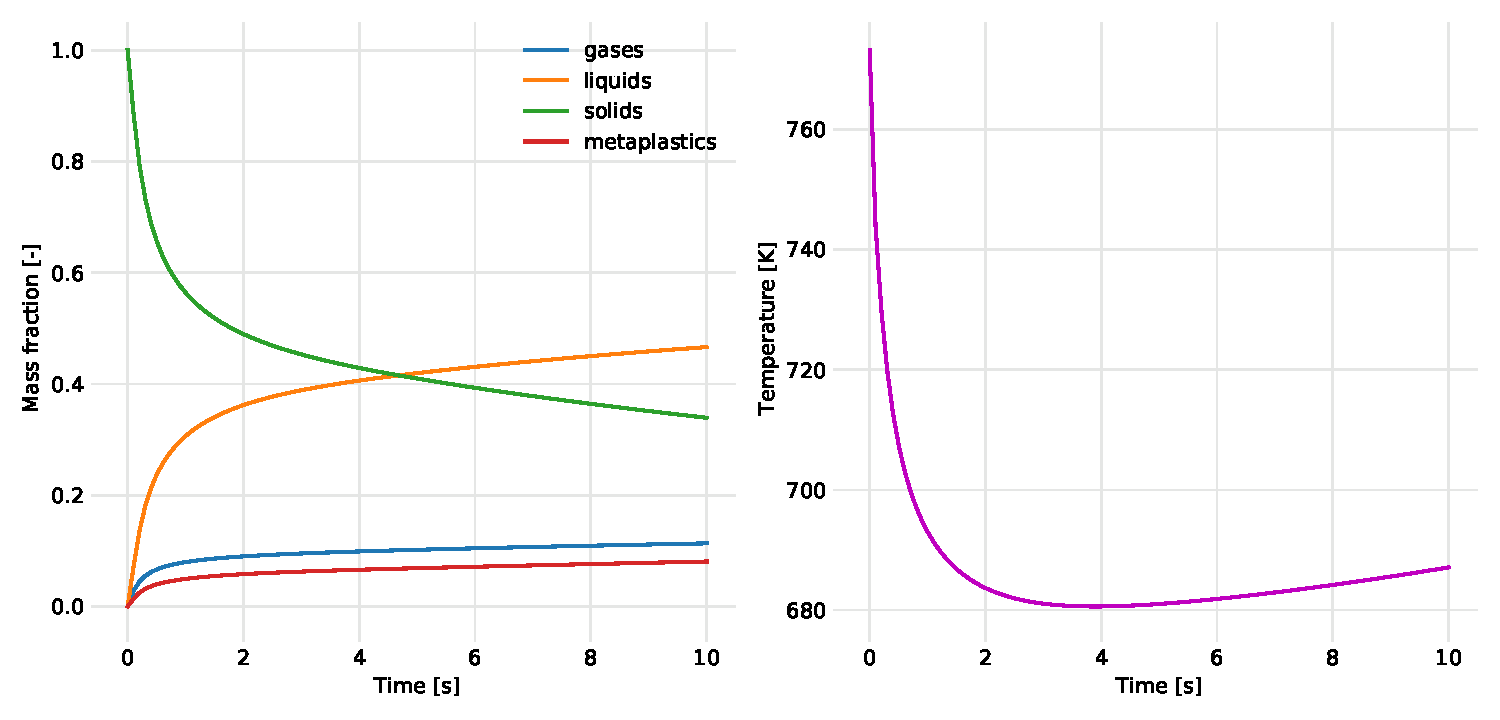
\includegraphics[width=\textwidth]{figures/blend3-case3-phases-temp-thermo.pdf}
        \caption{With thermodynamics.}
    \end{subfigure}
    \caption{Comparison of the gas, liquid, solid, and metaplastic phases in the batch reactor model for the Blend3 feedstock based on Case 3 biomass composition. Temperature profile represents reaction temperature.}
    \label{fig:blend3-case3-phases-temp}
\end{figure}

Figure \ref{fig:blend3-case3-final} depicts the final concentrations from the batch reactor model (with and without heats of reaction effects) after 10 seconds of reaction time at 500$^{\circ}$C. The most noticeable concentrations of gas species are CO and CO$_2$. Liquid products are mainly C$_6$H$_{10}$O$_5$, C$_6$H$_6$O$_3$, and H$_2$O. Without accounting for thermodynamics, char is the main solid species along with tannins. With thermodynamics, the major solid species are lignin components with lesser amounts of tannins, char, and unpyrolyzed cellulose. The main metaplastic species are G\{CH$_2$O\} and G\{COH$_2$\} for both scenarios with and without thermodynamic effects.

To maximize bio-oil yield from the entrained flow reactor, full conversion of the biomass to liquid products is needed. One way to accomplish this is to promote reactions that produce the liquid (condensable vapor) species. It is also desirable to decrease the solids yield from the reactor. According to the batch reactor model, the metaplastic species contribute considerably to the solid products. Enhancing the conversion of the metaplastics to gases and liquids could improve bio-oil yields and reduce solids production from the EFR.

\begin{figure}[H]
    \makebox[\textwidth][c]{
        \begin{subfigure}{1.3\textwidth}
            \centering
            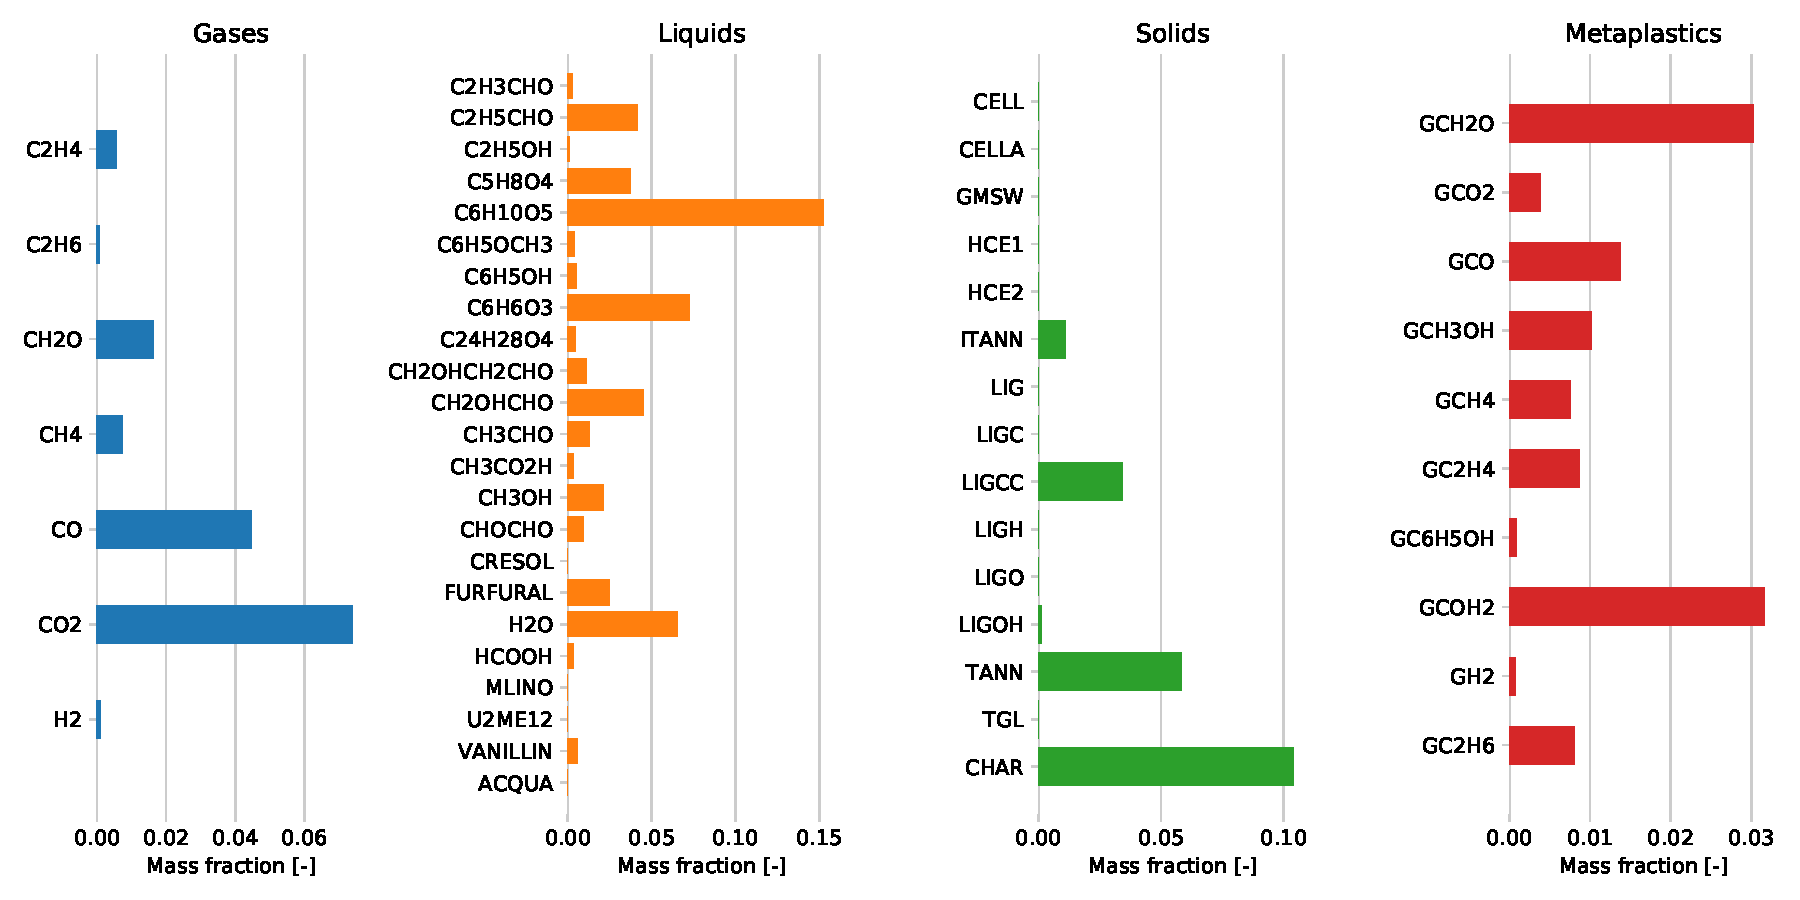
\includegraphics[width=\textwidth]{figures/blend3-case3-final.pdf}
            \caption{Without thermodynamics.}
        \end{subfigure}
    }
    \makebox[\textwidth][c]{
        \begin{subfigure}{1.3\textwidth}
            \centering
            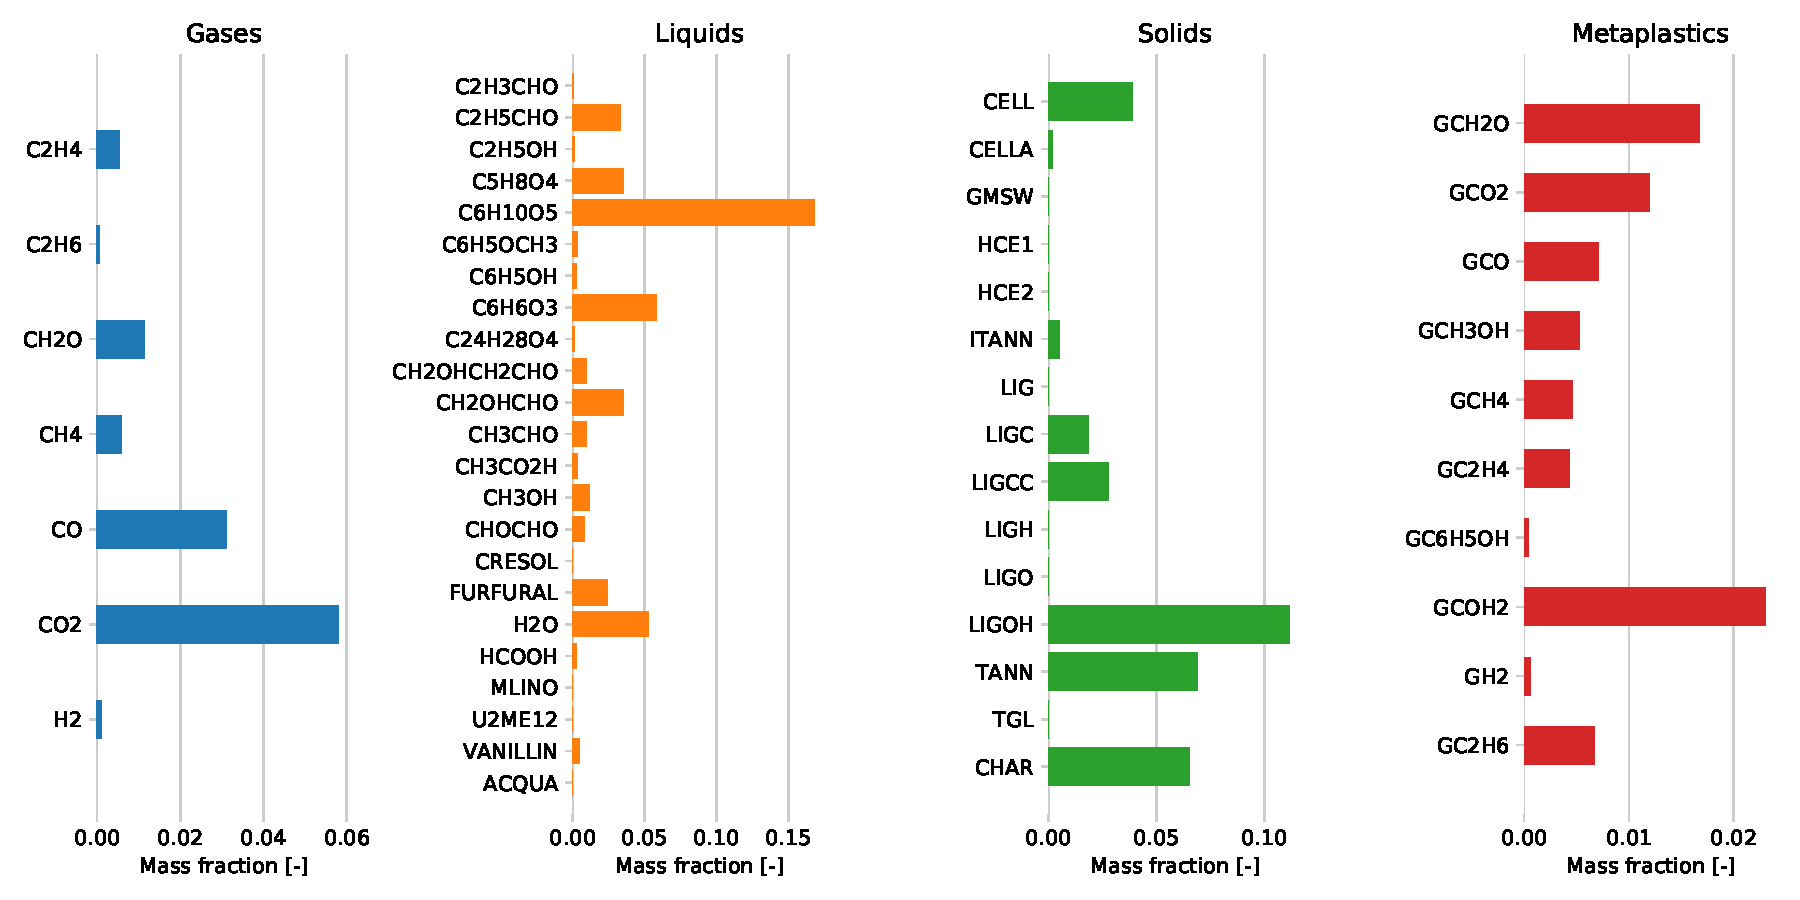
\includegraphics[width=\textwidth]{figures/blend3-case3-final-thermo.pdf}
            \caption{With thermodynamics.}
        \end{subfigure}
    }
    \caption{Final batch reactor concentrations for Blend3 feedstock based on Case 3 biomass composition.}
    \label{fig:blend3-case3-final}
\end{figure}

\subsection{Pyrolysis yields}

Conversion of the Blend3 feedstock along the length of the EFR using the Case 3 biomass composition and default reaction rates with the reduced-order model is shown in Figure \ref{fig:rom-yields1}. The EFR inlet is denoted by CSTR 0 while the outlet is CSTR 20 as labeled on the x-axis. Chemical species are lumped into gas, liquid, solid, and metaplastic phases. Reaction temperature and pressure in each CSTR are also shown in the figure. The final pyrolysis yields from the reduced-order model are given in Table \ref{tab:rom-yields1}. The yields are presented on a N$_2$ basis which includes the contribution of the nitrogen gas in the overall product and as a N$_2$ free basis which excludes the nitrogen gas fraction. Thermodynamic effects on the pyrolysis yields due to the heat of reaction ($\Delta$H) are also shown in the table.

A large portion of the product stream leaving the EFR is gas (mainly N$_2$) followed by liquid products. However, when considering only the biomass fraction, a majority of the products represent liquid species. By not including the heat of reaction effects ($\Delta$H off), the solid yield is decreased with an increase in liquid and gas production. This is likely due to the constant temperature applied to the biomass phase when $\Delta$H is ignored. Otherwise, the heat of reaction will have an endothermic effect on the biomass temperature thus decreasing its rate of conversion.

\begin{figure}[H]
    \centering
    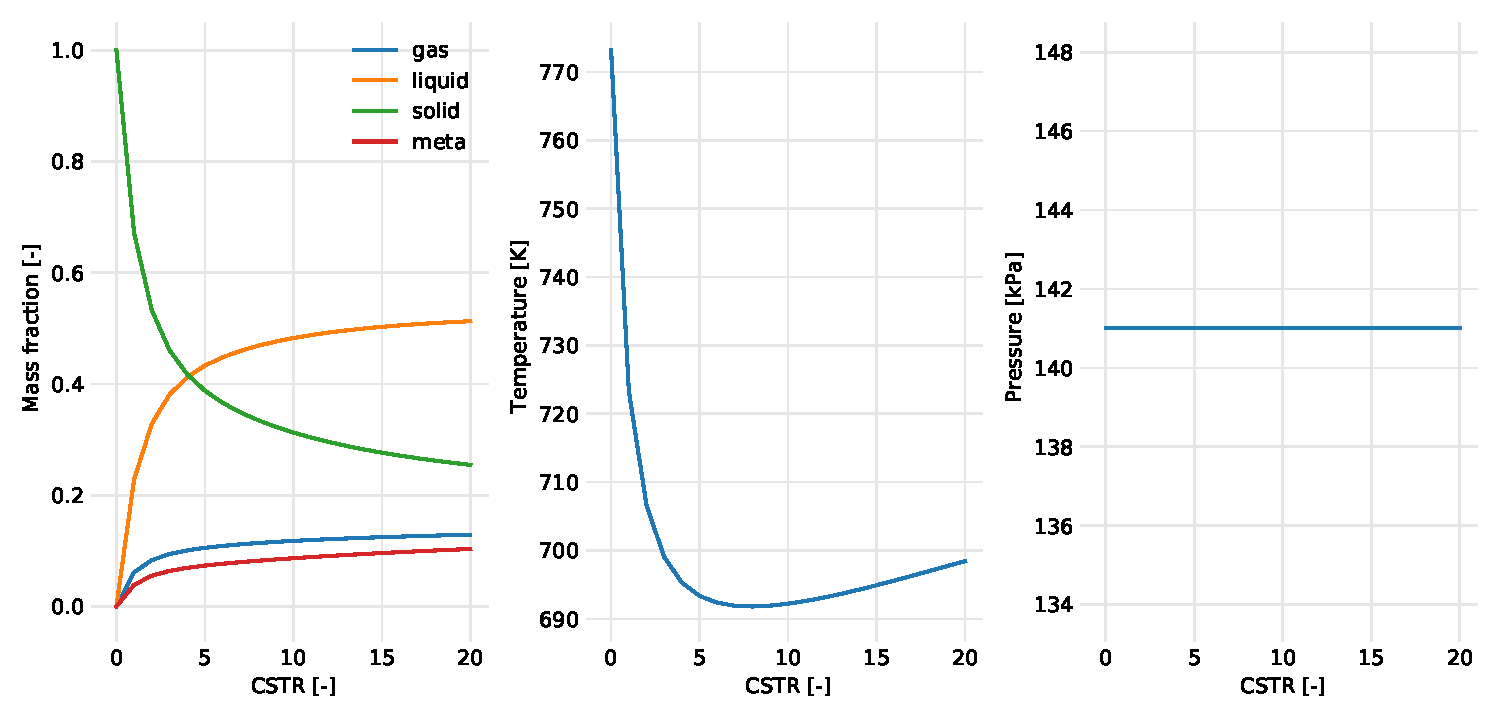
\includegraphics[width=\textwidth]{figures/rom-yields1.pdf}
    \caption{Blend3 feedstock conversion, temperature, and pressure from the reduced-order model using Case 3 biomass composition and default reaction rates. Results shown on a N$_2$ free basis with thermodynamic effects ($\Delta$H).}
    \label{fig:rom-yields1}
\end{figure}

\begin{table}[H]
    \centering
    \caption{Pyrolysis yields (\% mass) from the reduced-order model using Case 3 biomass composition and default reaction rates.}
    \label{tab:rom-yields1}
    \begin{tabular}{lrrrr}
        \toprule
        Pyrolysis yield & \multicolumn{2}{c}{N$_2$ basis} & \multicolumn{2}{c}{N$_2$ free basis} \\
        & $\Delta$H on & $\Delta$H off& $\Delta$H on & $\Delta$H off \\
        \midrule
        gas         & 56.5 & 57.7 & 12.9 & 15.4 \\
        liquid      & 25.6 & 26.6 & 51.3 & 53.1 \\
        solid       & 12.7 & 10.1 & 25.5 & 20.2 \\
        metaplastic & 5.2  & 5.7  & 10.3 & 11.3 \\
        total solid & 17.9 & 15.8 & 35.8 & 31.5 \\
        \bottomrule
    \end{tabular}
\end{table}

To improve conversion of the metaplastic species such that the total solids yield is decreased, the rates of reactions 22--31 in Table \ref{tab:chem-kinetics} were increased by T$^1$. Also, the Case 4 biomass composition is used to improve liquid yields as suggested from the sensitivity analysis mentioned earlier in the report. Using the faster metaplastic rates and Case 4 composition in the reduced-order model, Blend3 feedstock conversion along the EFR is shown in Figure \ref{fig:rom-yields2}. The final pyrolysis yields are given in Table \ref{tab:rom-yields2}. The largest decrease in metaplastic yields is observed for the constant temperature case ($\Delta$H off) which also provides an increase in gas and liquid yields.

\begin{figure}[H]
    \centering
    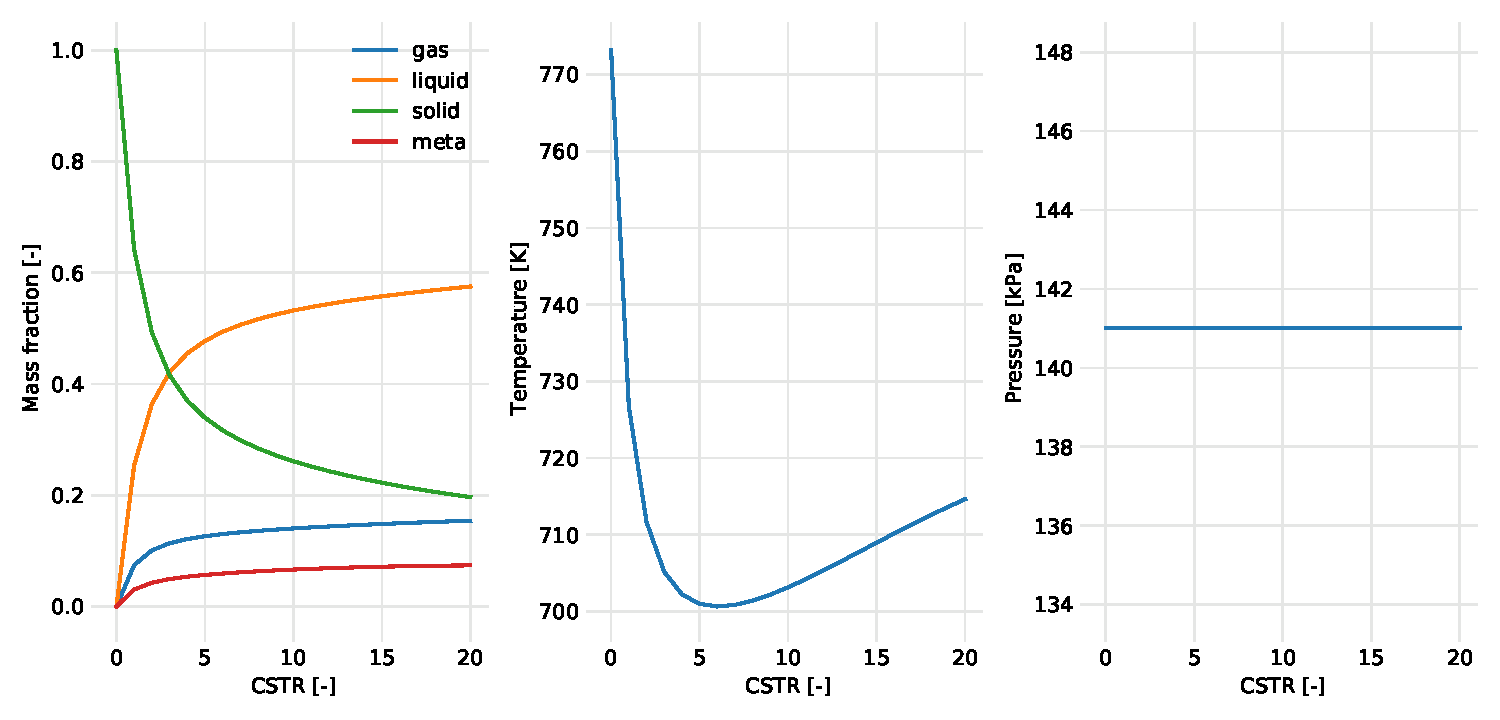
\includegraphics[width=\textwidth]{figures/rom-yields2.pdf}
    \caption{Blend3 feedstock conversion, temperature, and pressure from the reduced-order model using Case 4 biomass composition and increased reaction rates for metaplastic species. Results shown on a N$_2$ free basis with thermodynamic effects ($\Delta$H).}
    \label{fig:rom-yields2}
\end{figure}

\begin{table}[H]
    \centering
    \caption{Pyrolysis yields (\% mass) from the reduced-order model using Case 4 biomass composition and increased reaction rates for metaplastic species.}
    \label{tab:rom-yields2}
    \begin{tabular}{lrrrr}
        \toprule
        Pyrolysis yield & \multicolumn{2}{c}{N$_2$ basis} & \multicolumn{2}{c}{N$_2$ free basis} \\
        & $\Delta$H on & $\Delta$H off& $\Delta$H on & $\Delta$H off \\
        \midrule
        gas         & 57.7 & 59.5 & 15.4 & 19.0 \\
        liquid      & 28.8 & 31.1 & 57.5 & 62.2 \\
        solid       &  9.8 &  7.4 & 19.7 & 14.8 \\
        metaplastic &  3.7 &  2.0 &  7.4 &  3.9 \\
        total solid & 13.5 &  9.4 & 27.1 & 18.7 \\
        \bottomrule
    \end{tabular}
\end{table}

Finally, a comparison of the pyrolysis yields from the EFR data and the reduced-order model for the Blend3 feedstock is given in Table \ref{tab:blend3-yields}. To get favorable results from the model, the thermodynamic effects were excluded to ensure a constant reaction temperature of the biomass phase. Using the Case 3 biomass composition, total liquid yields from the model were about 10\% lower than measured values. Better results were obtained using the Case 4 composition which excludes the tannin fraction in favor of triglycerides. This approach provides a less than 3\% difference between measured values and model results for the total liquids yield. The Case 5 biomass composition improves the model's total liquid and char yield estimates at the expense of the gas yield prediction. However, the mass balance from the EFR measurements is 96\%; consequently, 4\% of the pyrolysis products are not accounted in the measured data. This could account for some of the discrepancies between the model results and measured values.

\begin{table}[H]
    \centering
    \caption{Comparison of the EFR Blend3 feedstock yields to the reduced-order model. Values reported as \% mass and N$_2$ free basis. Cases represent model yields without thermodynamic effects ($\Delta$H off) and increased metaplastic reaction rates.}
    \label{tab:blend3-yields}
    \begin{tabular}{lrrrr}
        \toprule
        Pyrolysis yields & Exp. & Case 3 & Case 4 & Case 5 \\
        \midrule
        total liquid & 64.9 & 55.6  & 62.2  & 63.4  \\
        char         & 13.9 & 25.1  & 18.8  & 16.0  \\
        gas          & 17.2 & 19.3  & 19.0  & 20.6  \\
        sum          & 96.0 & 100.0 & 100.0 & 100.0 \\
        \bottomrule
    \end{tabular}
\end{table}
